\documentclass{beamer}

% For more themes, color themes and font themes, see:
% http://deic.uab.es/~iblanes/beamer_gallery/index_by_theme.html
%
\mode<presentation>
{
  \usetheme{Madrid}       % or try default, Darmstadt, Warsaw, ...
  \usecolortheme{crane} % or try albatross, beaver, crane, ...
  \usefonttheme{serif}    % or try default, structurebold, ...
  \setbeamertemplate{navigation symbols}{}
  \setbeamertemplate{caption}[numbered]
} 

\usepackage{tikz}
\usetikzlibrary{decorations.markings,angles}
\usepackage{tikz-3dplot} 

\usepackage{amsmath}


\begin{document}



\begin{frame}{Magnetic field measurements}

 first vector
magnetic field inferences along an individual, resolved coronal
loop structure extending up to heights of 70 Mm (0.1 RSun ), and
the first polarimetric measurements of coronal loops located on
disk

off limb measurements

Tomczyk et al. 2008
 
\begin{itemize}
\item azimuth of the magnetic field from linear polarization(ambiguity in orientation): 

$\phi$ = 0.5 arctan(U/Q)



\item strength of L.O.S  magnetic field from zeeman shift
\end{itemize}

\end{frame}

\begin{frame}{Magnetic field measurements}
 
\begin{figure}[H]
 \centering
 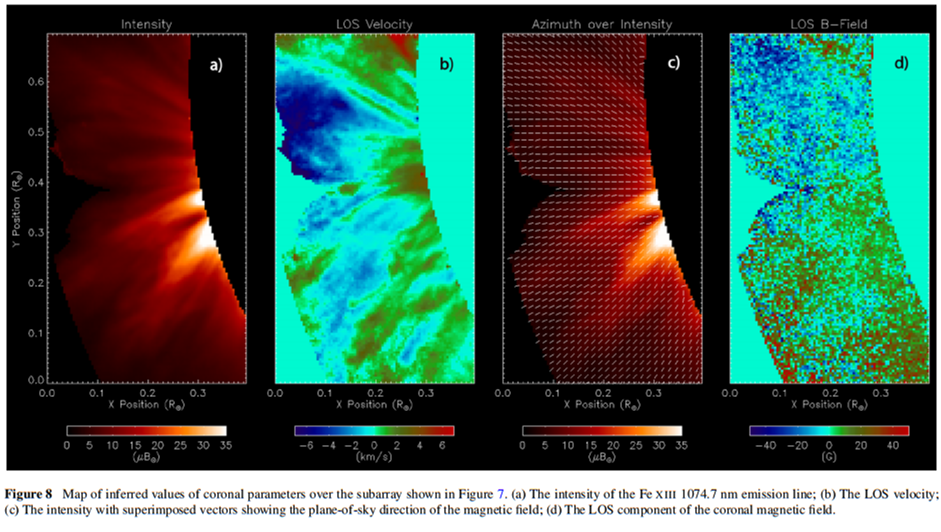
\includegraphics[scale=0.35]{t1.png}
\caption{Tomczyk et al. 2008 measurements}
\end{figure}



\end{frame}

\end{document}
